\chapter{Dataset Understanding}

\section{Overview of MIMIC-IV}
The \textbf{Medical Information Mart for Intensive Care (MIMIC-IV)} is a large, freely accessible electronic health record (EHR) dataset developed by the Beth Israel Deaconess Medical Center (BIDMC) and the Massachusetts Institute of Technology (MIT). It spans clinical stays from 2008 to 2019 and contains comprehensive, de-identified data on hospital admissions, including demographics, clinical notes, laboratory values, prescriptions, and billing codes~\cite{johnson2023mimicivscidata,nguyen2023mimicivicd}. Key modules include:
\begin{itemize}
    \item \texttt{hosp}: Hospital-wide data (e.g., \texttt{admissions}, \texttt{patients}, \texttt{diagnoses\_icd}).
    \item \texttt{icu}: ICU-specific charting data (e.g., \texttt{chartevents}).
    \item \texttt{ed}: Emergency department data.
    \item \texttt{note}: De-identified textual notes, including \texttt{discharge}.
    \item \texttt{cxr}: Linking data for chest X-ray images (MIMIC-CXR).
\end{itemize}
For automated ICD coding from discharge summaries, we focus on:
\begin{itemize}
    \item \texttt{patients} (in \textit{hosp}) for demographics (\texttt{anchor\_age}, \texttt{anchor\_year\_group}).
    \item \texttt{admissions} (in \textit{hosp}) for hospital-stay details (\texttt{hadm\_id}, \texttt{admittime}, \texttt{dischtime}).
    \item \texttt{diagnoses\_icd} (in \textit{hosp}) for billed ICD-9 or ICD-10 diagnoses.
    \item \texttt{discharge} (in \textit{note}) for textual discharge summaries.
\end{itemize}

\vspace{0.2cm}
\noindent
Below, we highlight key \textbf{SQL queries} run on \texttt{DuckDB}, their \textbf{results}, and \textbf{plots} illustrating the dataset's characteristics.

\section{Key SQL Queries and Results}

\subsection{Patient and Admission Counts}
\begin{verbatim}
SELECT
    COUNT(*) AS total_rows_in_patients,
    COUNT(DISTINCT subject_id) AS num_unique_patients
FROM mimic.patients;
\end{verbatim}
\begin{center}
\begin{tabular}{l|l}
\hline
\texttt{total\_rows\_in\_patients} & \texttt{num\_unique\_patients} \\
\hline
364627 & 364627 \\
\hline
\end{tabular}
\end{center}
So there are \textbf{364,627 unique patients} in the \texttt{patients} table.

\begin{verbatim}
SELECT
    COUNT(*) AS total_rows_in_admissions,
    COUNT(DISTINCT hadm_id) AS num_unique_admissions
FROM mimic.admissions;
\end{verbatim}
\begin{center}
\begin{tabular}{l|l}
\hline
\texttt{total\_rows\_in\_admissions} & \texttt{num\_unique\_admissions} \\
\hline
546028 & 546028 \\
\hline
\end{tabular}
\end{center}
Hence, \textbf{546,028 unique admissions} exist in MIMIC-IV.

\subsection{Multiple Admissions per Patient}
\begin{verbatim}
SELECT subject_id, COUNT(*) AS num_admissions
FROM mimic.admissions
GROUP BY subject_id
HAVING COUNT(*) > 1
ORDER BY num_admissions DESC
LIMIT 5;
\end{verbatim}
\begin{center}
\begin{tabular}{l|l}
\hline
\texttt{subject\_id} & \texttt{num\_admissions} \\
\hline
15496609 & 238 \\
15464144 & 185 \\
10714009 & 163 \\
16662316 & 142 \\
14394983 & 138 \\
\hline
\end{tabular}
\end{center}
Some patients have very frequent hospital stays (\(>100\) admissions).

\subsection{Discharge Summaries}
\begin{verbatim}
SELECT COUNT(*) AS total_discharge_notes
FROM mimic.discharge;
\end{verbatim}
\begin{center}
\begin{tabular}{l}
\hline
\texttt{total\_discharge\_notes} \\
\hline
331793 \\
\hline
\end{tabular}
\end{center}
Thus, \textbf{331,793 discharge summaries} are available.

\begin{verbatim}
SELECT
    (SELECT COUNT(DISTINCT hadm_id) FROM mimic.admissions) AS total_admissions,
    (SELECT COUNT(DISTINCT hadm_id) FROM mimic.discharge)  AS hadm_with_discharge,
    (SELECT COUNT(DISTINCT hadm_id) FROM mimic.admissions
     WHERE hadm_id NOT IN (
         SELECT DISTINCT hadm_id FROM mimic.discharge
     )
    ) AS hadm_without_discharge;
\end{verbatim}
\begin{center}
\begin{tabular}{l|l|l}
\hline
\texttt{total\_admissions} & \texttt{hadm\_with\_discharge} & \texttt{hadm\_without\_discharge} \\
\hline
546028 & 331793 & 214296 \\
\hline
\end{tabular}
\end{center}
Hence \(\sim214{,}296\) admissions have no final discharge note.

\subsection{Word Count in Discharge Summaries}
\begin{verbatim}
SELECT
    PERCENTILE_CONT(0.5)
        WITHIN GROUP (ORDER BY (LENGTH(text) - LENGTH(REPLACE(text, ' ', '')) + 1))
      AS median_word_count,
    PERCENTILE_CONT(0.9)
      WITHIN GROUP (ORDER BY (LENGTH(text) - LENGTH(REPLACE(text, ' ', '')) + 1))
    AS p90_word_count,
    PERCENTILE_CONT(0.99)
    WITHIN GROUP (ORDER BY (LENGTH(text) - LENGTH(REPLACE(text, ' ', '')) + 1))
    AS p99_word_count
FROM mimic.discharge;
\end{verbatim}
\begin{center}
\begin{tabular}{l|l|l}
\hline
\texttt{median\_word\_count} & \texttt{p90\_word\_count} & \texttt{p99\_word\_count} \\
\hline
1556 & 2556 & 3986 \\
\hline
\end{tabular}
\end{center}
Median discharge notes contain \textbf{\(\approx1{,}556\) words}, with 1\% of notes exceeding \(\approx3{,}986\) words.

\subsection{ICD-9 vs. ICD-10}
\begin{verbatim}
SELECT
    icd_version,
    COUNT(*) AS code_assignments
FROM mimic.diagnoses_icd
GROUP BY icd_version
ORDER BY code_assignments DESC;
\end{verbatim}
\begin{center}
\begin{tabular}{l|l}
\hline
\texttt{icd\_version} & \texttt{code\_assignments} \\
\hline
10 & 3455747 \\
9  & 2908741 \\
\hline
\end{tabular}
\end{center}
We have \(\sim3.46\)M ICD-10 assignments and \(\sim2.91\)M ICD-9.

\begin{verbatim}
SELECT icd_code, COUNT(*) AS freq
FROM mimic.diagnoses_icd
WHERE icd_version = 10
GROUP BY icd_code
ORDER BY freq DESC
LIMIT 10;
\end{verbatim}
\begin{center}
\begin{tabular}{l|l}
\hline
\texttt{icd\_code} & \texttt{freq} \\
\hline
E785   & 84570  \\
I10    & 83775  \\
Z87891 & 62806  \\
K219   & 56157  \\
F329   & 41876  \\
I2510  & 41550  \\
F419   & 38911  \\
N179   & 35884  \\
Z20822 & 33113  \\
Z7901  & 30957  \\
\hline
\end{tabular}
\end{center}
Common chronic diseases like hyperlipidemia (\texttt{E785}) and hypertension (\texttt{I10}) appear most frequently.

\subsection{Unique Codes and Rare-Code Challenge}
\begin{verbatim}
SELECT icd_version,
       COUNT(DISTINCT icd_code) AS num_unique_codes
FROM mimic.diagnoses_icd
GROUP BY icd_version;
\end{verbatim}
\begin{center}
\begin{tabular}{l|l}
\hline
\texttt{icd\_version} & \texttt{num\_unique\_codes} \\
\hline
10 & 19440 \\
9  & 9143  \\
\hline
\end{tabular}
\end{center}
MIMIC-IV has \textbf{19,440 ICD-10 codes}. Many are rare:

\begin{verbatim}
WITH code_counts AS (
    SELECT icd_code, COUNT(*) AS freq
    FROM mimic.diagnoses_icd
    WHERE icd_version = 10
    GROUP BY icd_code
)
SELECT COUNT(*) AS codes_under_5_occurrences
FROM code_counts
WHERE freq < 5;
\end{verbatim}
\begin{center}
\begin{tabular}{l}
\hline
\texttt{codes\_under\_5\_occurrences} \\
\hline
9217 \\
\hline
\end{tabular}
\end{center}
Thus, \(\approx9{,}217\) ICD-10 codes appear fewer than 5 times (long-tail distribution).

\subsection{Average Number of ICD-10 Codes per Admission}
\begin{verbatim}
WITH code_counts AS (
    SELECT hadm_id,
           COUNT(DISTINCT icd_code) AS code_count
    FROM mimic.diagnoses_icd
    WHERE icd_version = 10
    GROUP BY hadm_id
)
SELECT AVG(code_count) AS avg_icd10_codes_per_adm
FROM code_counts;
\end{verbatim}
\begin{center}
\begin{tabular}{l}
\hline
\texttt{avg\_icd10\_codes\_per\_adm} \\
\hline
13.584911371704203 \\
\hline
\end{tabular}
\end{center}
On average, \(\sim13.6\) ICD-10 codes per admission.

\section{Visual Exploration of Data}

\begin{figure}[ht!]
    \centering
    \begin{subfigure}{0.42\textwidth}
        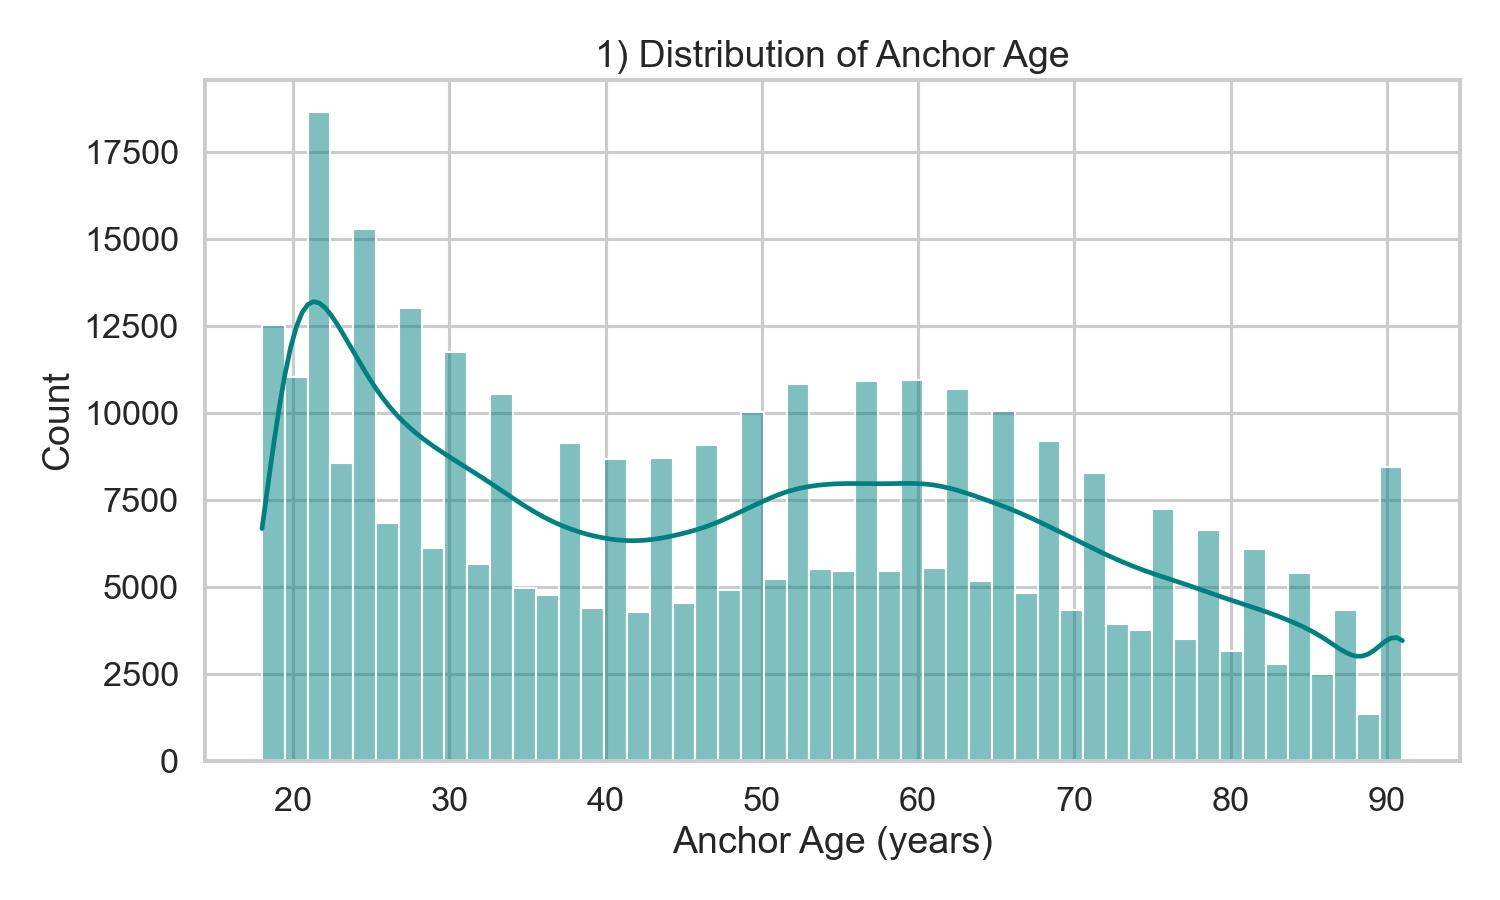
\includegraphics[width=\linewidth]{mimic_plots/plot1.jpg}
    \end{subfigure}\hfill
    \begin{subfigure}{0.54\textwidth}
        \footnotesize
        \textbf{(1) Distribution of Anchor Age}\newline
        1) The histogram shows a right-skewed age distribution, with more patients in their 20s and 30s.\newline
        2) KDE overlay highlights ages up to the capped 91 group.\newline
        3) Frequency gradually declines after middle age, with a small uptick around 90--91.
    \end{subfigure}
    \caption{Left: Distribution of Anchor Age. Right: Description.}
    \label{fig:plot1}
\end{figure}

\begin{figure}[ht!]
    \centering
    \begin{subfigure}{0.42\textwidth}
        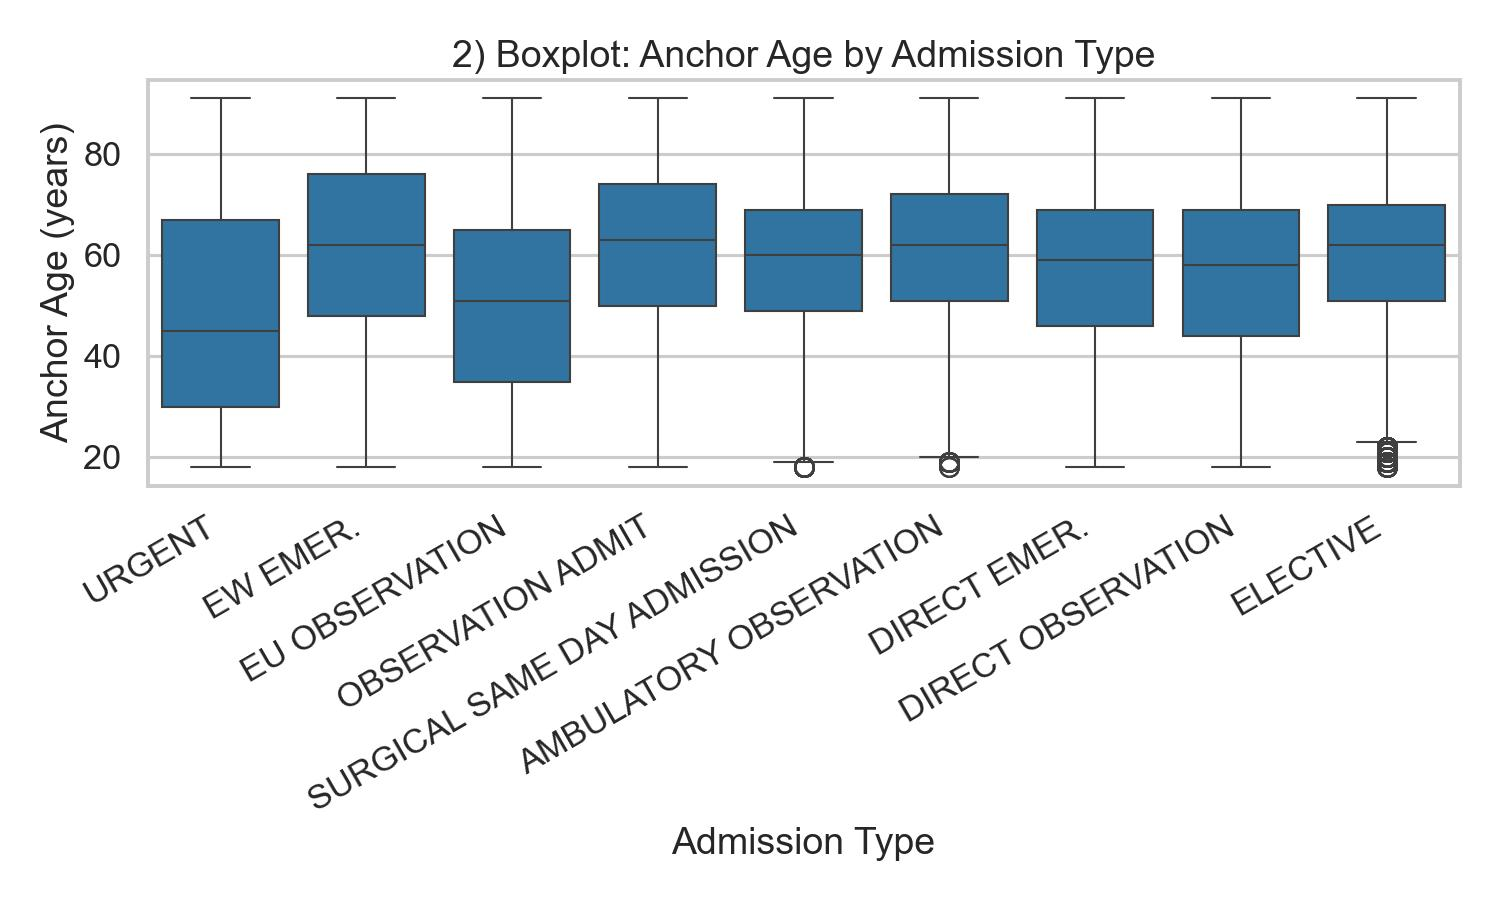
\includegraphics[width=\linewidth]{mimic_plots/plot2.jpg}
    \end{subfigure}\hfill
    \begin{subfigure}{0.54\textwidth}
        \footnotesize
        \textbf{(2) Boxplot: Anchor Age by Admission Type}\newline
        1) Shows median and spread of anchor age across each admission type.\newline
        2) Some types (e.g. “EW EMER.”) cover a broader range, while “ELECTIVE” is narrower.\newline
        3) Outliers appear as points, indicating unusual or extreme anchor ages for some admissions.
    \end{subfigure}
    \caption{Left: Boxplot for Anchor Age vs. Admission Type. Right: Description.}
    \label{fig:plot2}
\end{figure}

\begin{figure}[ht!]
    \centering
    \begin{subfigure}{0.42\textwidth}
        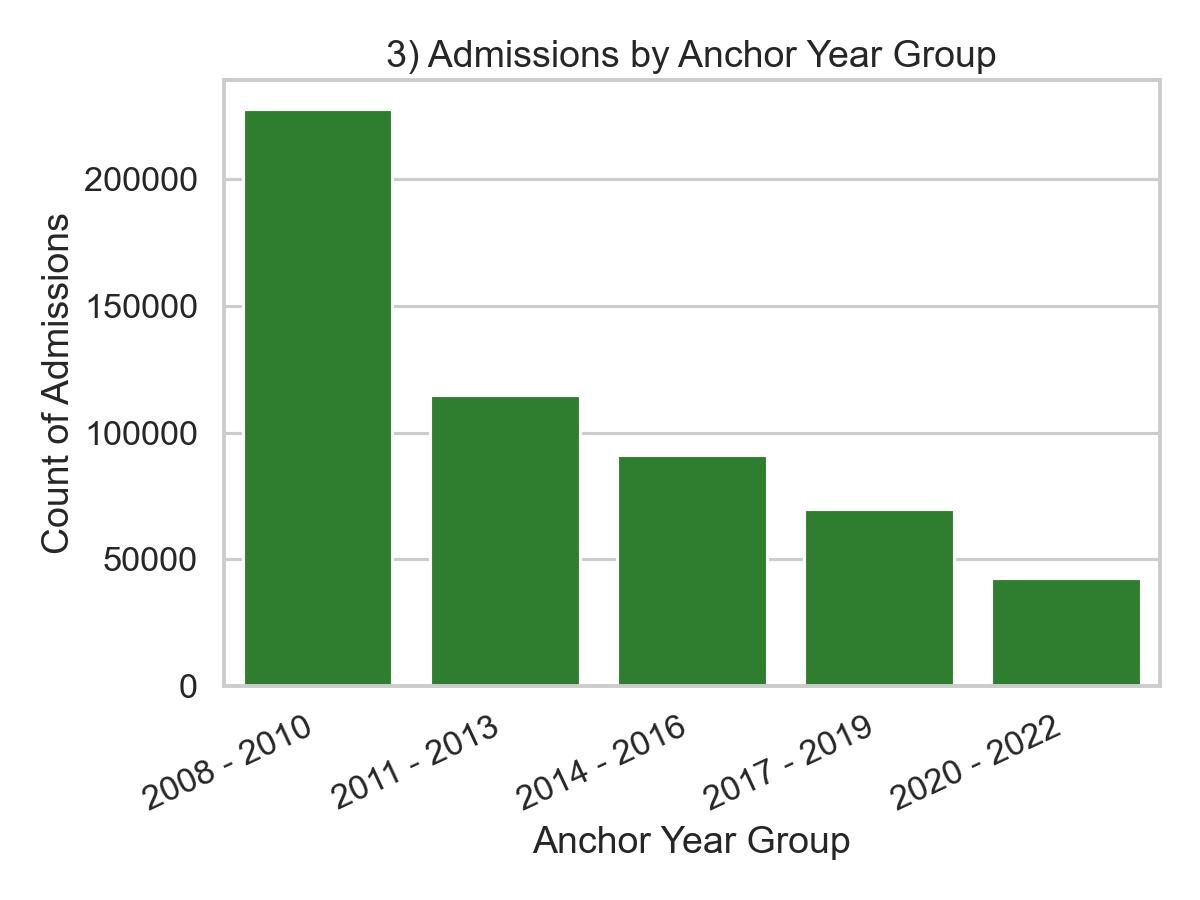
\includegraphics[width=\linewidth]{mimic_plots/plot3.jpg}
    \end{subfigure}\hfill
    \begin{subfigure}{0.54\textwidth}
        \footnotesize
        \textbf{(3) Admissions by Anchor Year Group}\newline
        1) A bar chart capturing the count of admissions over 5 approximate time intervals.\newline
        2) 2008--2010 and 2011--2013 are noticeably higher, possibly reflecting data coverage.\newline
        3) Later intervals show fewer admissions, hinting at different data capture or hospital volumes.
    \end{subfigure}
    \caption{Left: Admissions distribution by anchor year group. Right: Description.}
    \label{fig:plot3}
\end{figure}

\begin{figure}[ht!]
    \centering
    \begin{subfigure}{0.42\textwidth}
        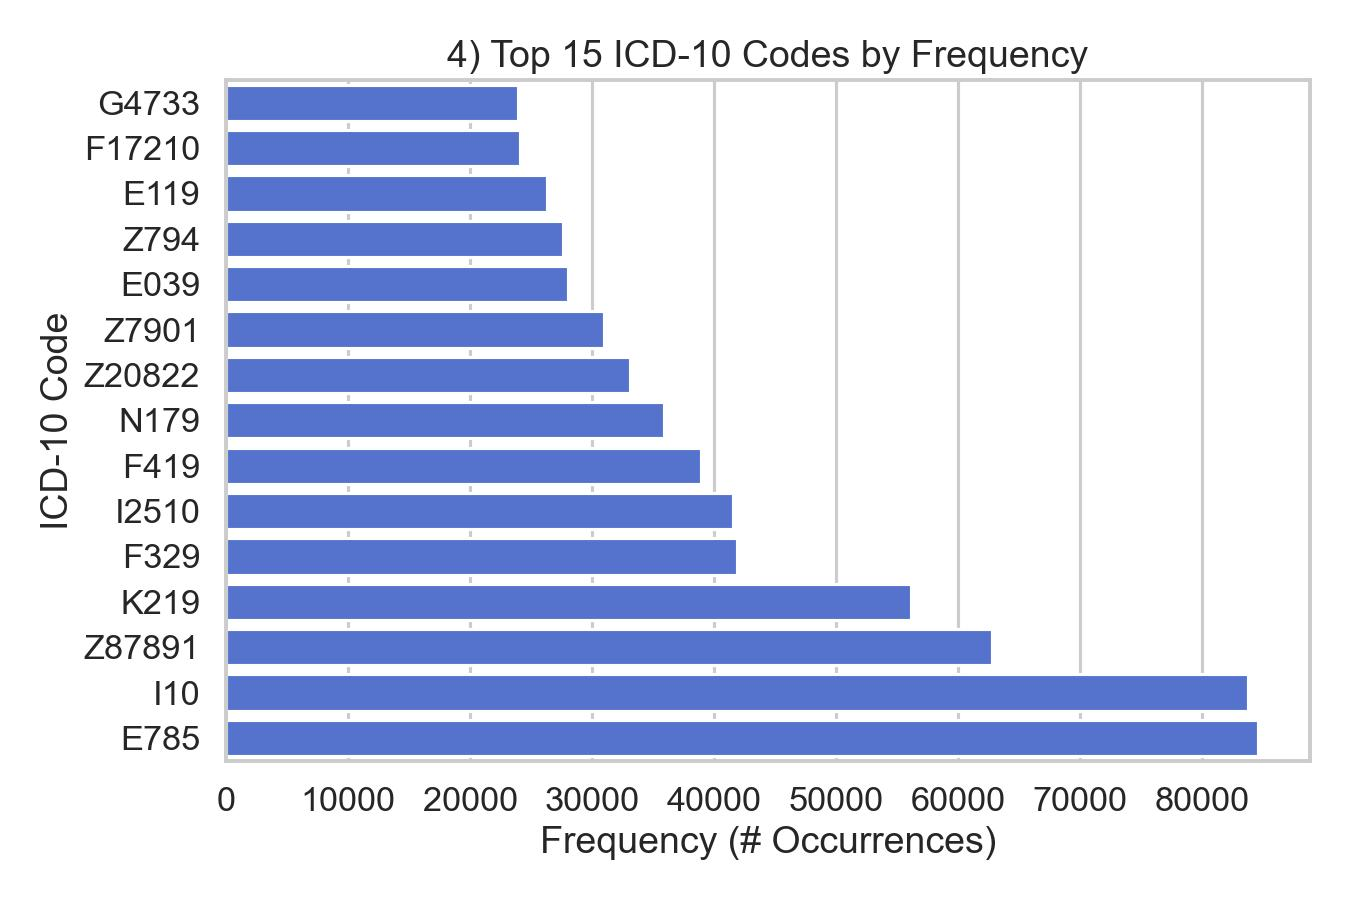
\includegraphics[width=\linewidth]{mimic_plots/plot4.jpg}
    \end{subfigure}\hfill
    \begin{subfigure}{0.54\textwidth}
        \footnotesize
        \textbf{(4) Top 15 ICD-10 Codes by Frequency}\newline
        1) Horizontal bar chart listing the most frequent ICD-10 codes.\newline
        2) E785 (Hyperlipidemia) and I10 (Hypertension) top the chart.\newline
        3) Chronic conditions like diabetes (E119) also feature prominently.
    \end{subfigure}
    \caption{Left: Bar plot of top 15 ICD-10 codes. Right: Description.}
    \label{fig:plot4}
\end{figure}

\begin{figure}[ht!]
    \centering
    \begin{subfigure}{0.42\textwidth}
        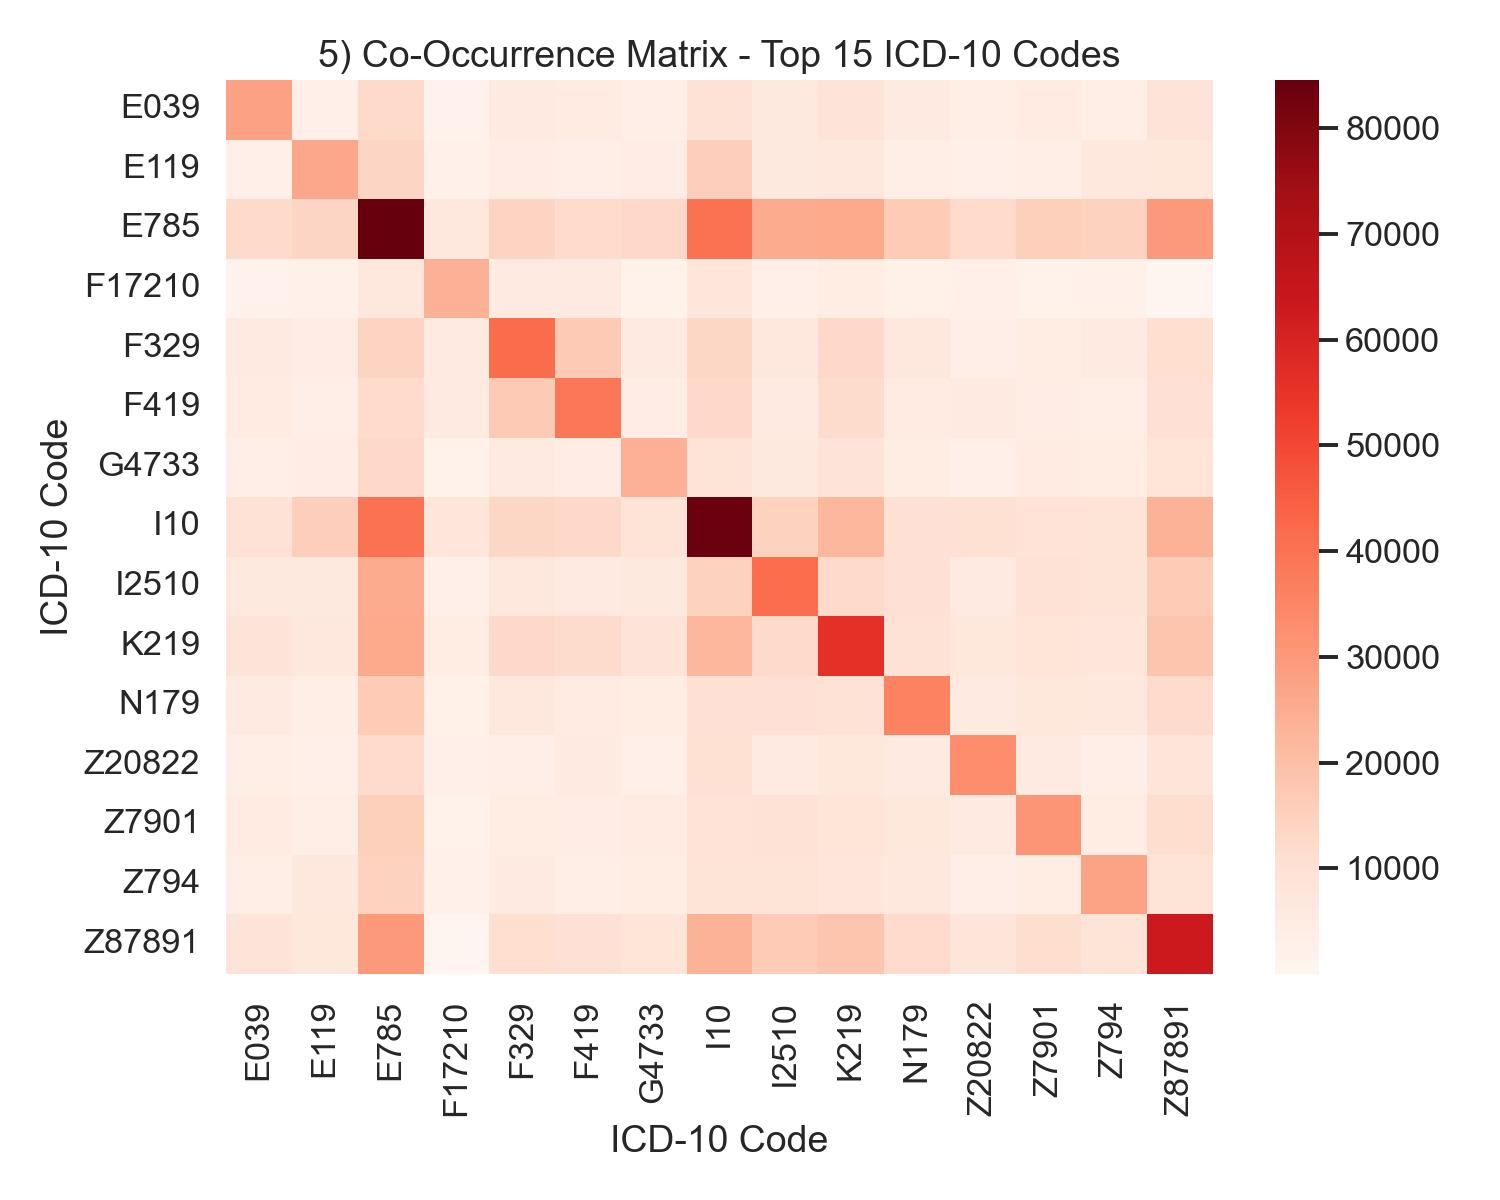
\includegraphics[width=\linewidth]{mimic_plots/plot5.jpg}
    \end{subfigure}\hfill
    \begin{subfigure}{0.54\textwidth}
        \footnotesize
        \textbf{(5) Co-Occurrence Matrix -- Top 15 ICD-10 Codes}\newline
        1) Heatmap showing how often two specific codes appear together.\newline
        2) Darker squares indicate strong co-occurrence (e.g., E785 with I10).\newline
        3) Points to common comorbidity clusters among high-frequency codes.
    \end{subfigure}
    \caption{Left: Heatmap of code co-occurrences. Right: Description.}
    \label{fig:plot5}
\end{figure}

\begin{figure}[ht!]
    \centering
    \begin{subfigure}{0.42\textwidth}
        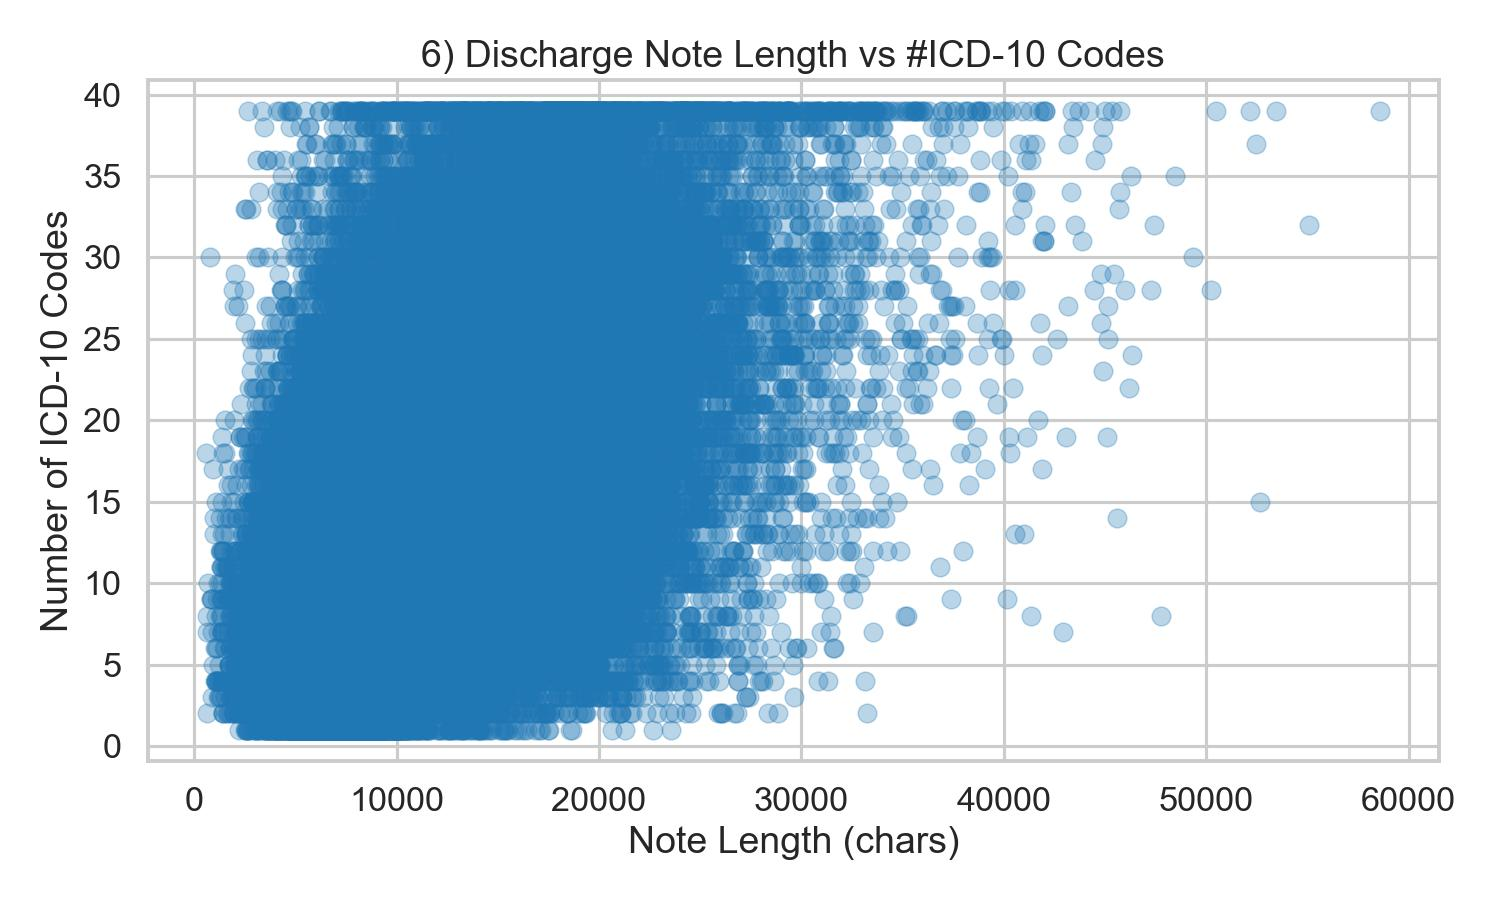
\includegraphics[width=\linewidth]{mimic_plots/plot6.jpg}
    \end{subfigure}\hfill
    \begin{subfigure}{0.54\textwidth}
        \footnotesize
        \textbf{(6) Discharge Note Length vs. \# ICD-10 Codes}\newline
        1) A scatterplot comparing how many codes an admission has vs. note length (chars).\newline
        2) There's a positive trend: very long notes often have 20+ codes.\newline
        3) The bulk of admissions cluster below 20k characters but still can have 5--15 codes.
    \end{subfigure}
    \caption{Left: Scatterplot of note length vs. number of ICD-10 codes. Right: Description.}
    \label{fig:plot6}
\end{figure}

\begin{figure}[ht!]
    \centering
    \begin{subfigure}{0.42\textwidth}
        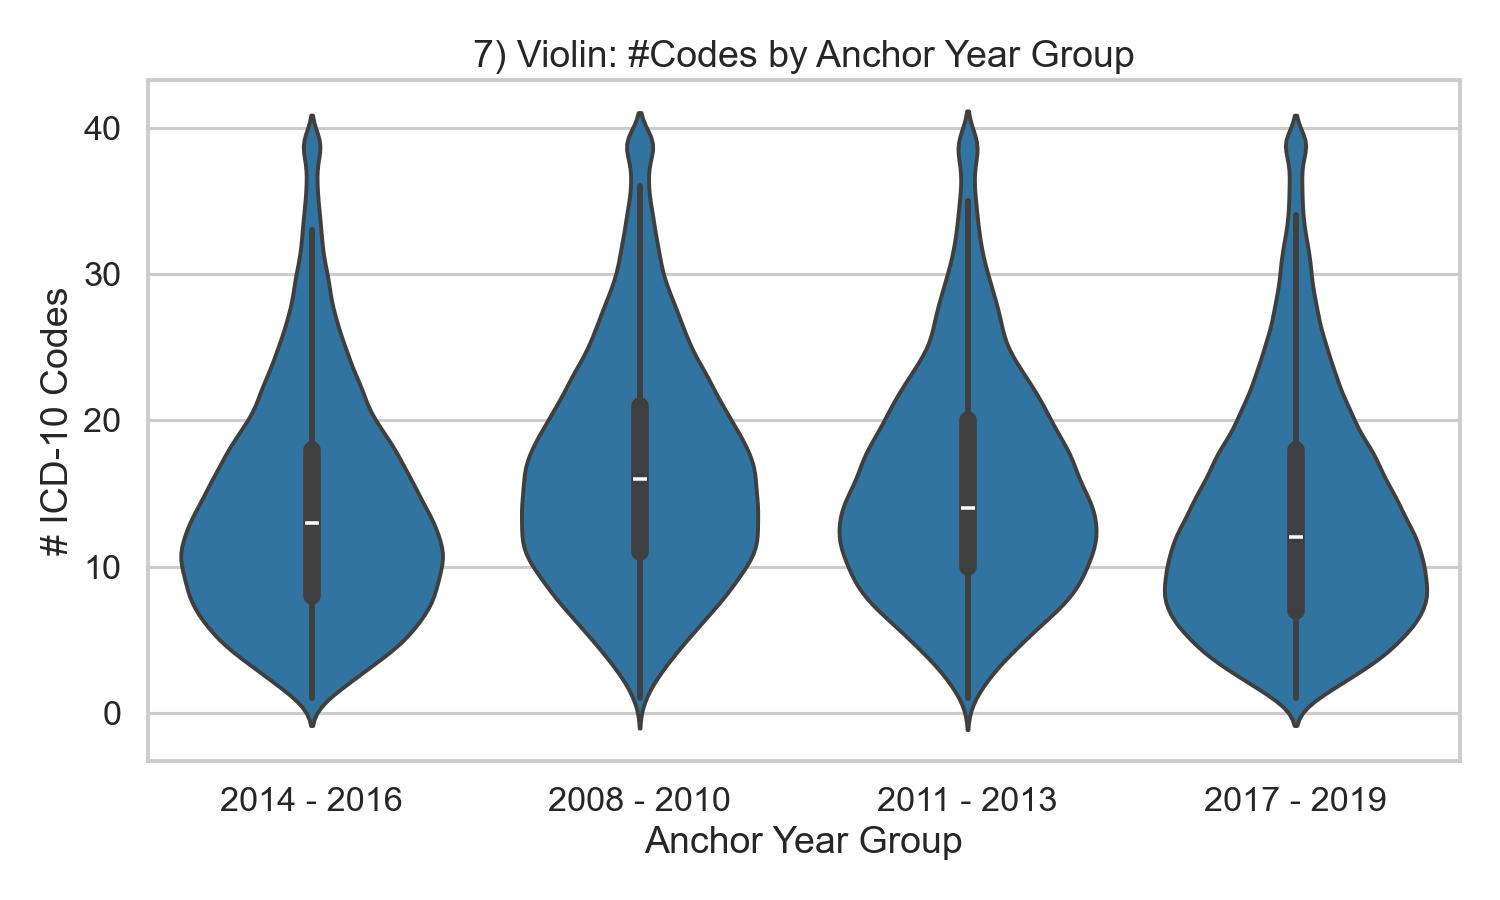
\includegraphics[width=\linewidth]{mimic_plots/plot7.jpg}
    \end{subfigure}\hfill
    \begin{subfigure}{0.54\textwidth}
        \footnotesize
        \textbf{(7) Violin: \# Codes by Anchor Year Group}\newline
        1) Violin plots indicate distribution shapes of code counts for each year group.\newline
        2) The median is shown by a white dot; thick black bar is the IQR.\newline
        3) Some groups exhibit very wide “tails,” reflecting occasional high-code admissions.
    \end{subfigure}
    \caption{Left: Violin plot of code counts across anchor year groups. Right: Description.}
    \label{fig:plot7}
\end{figure}

\begin{figure}[ht!]
    \centering
    \begin{subfigure}{0.42\textwidth}
        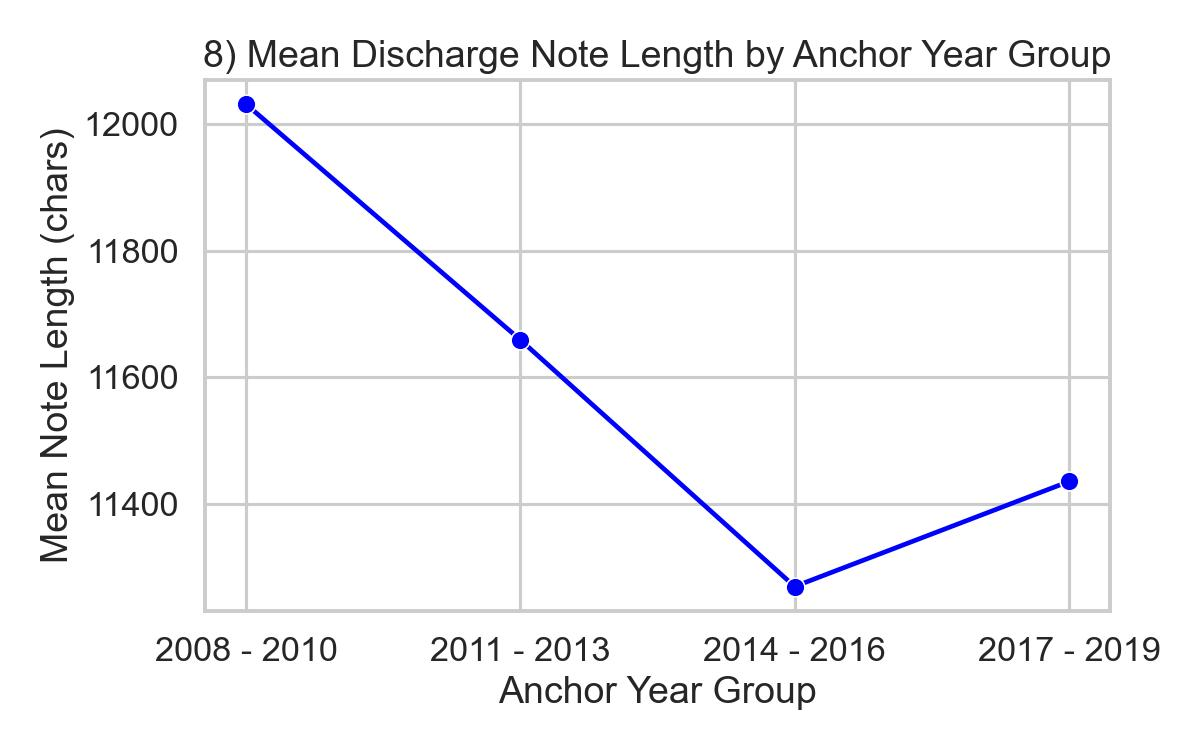
\includegraphics[width=\linewidth]{mimic_plots/plot8.jpg}
    \end{subfigure}\hfill
    \begin{subfigure}{0.54\textwidth}
        \footnotesize
        \textbf{(8) Mean Discharge Note Length by Anchor Year Group}\newline
        1) A line plot tracking average note length over time intervals.\newline
        2) Highest in 2008--2010, dipping by 2014--2016, then slight rebound.\newline
        3) Suggests evolving documentation practices or EHR usage over the years.
    \end{subfigure}
    \caption{Left: Line plot of average note length vs. anchor year group. Right: Description.}
    \label{fig:plot8}
\end{figure}

\begin{figure}[ht!]
    \centering
    \begin{subfigure}{0.42\textwidth}
        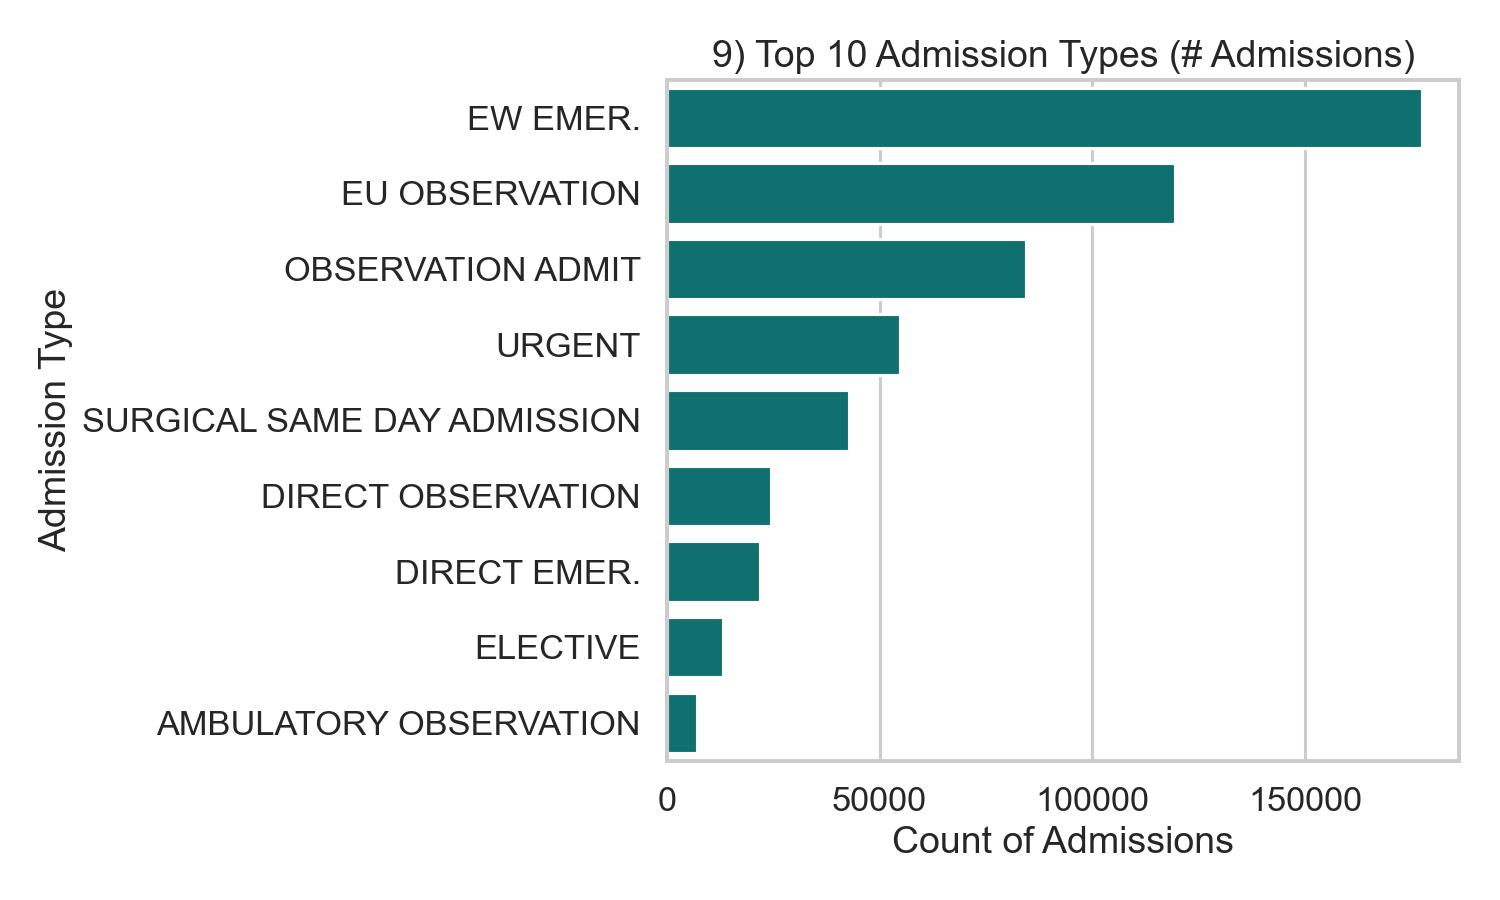
\includegraphics[width=\linewidth]{mimic_plots/plot9.jpg}
    \end{subfigure}\hfill
    \begin{subfigure}{0.54\textwidth}
        \footnotesize
        \textbf{(9) Top 10 Admission Types (\# Admissions)}\newline
        1) A horizontal bar ranking the most frequent admission types.\newline
        2) “EW EMER.” (Emergency) is the largest slice of admissions.\newline
        3) “AMBULATORY OBSERVATION” ranks lowest among the top 10 but is still substantial.
    \end{subfigure}
    \caption{Left: Bar plot of top 10 admission types by volume. Right: Description.}
    \label{fig:plot9}
\end{figure}

\begin{figure}[ht!]
    \centering
    \begin{subfigure}{0.42\textwidth}
        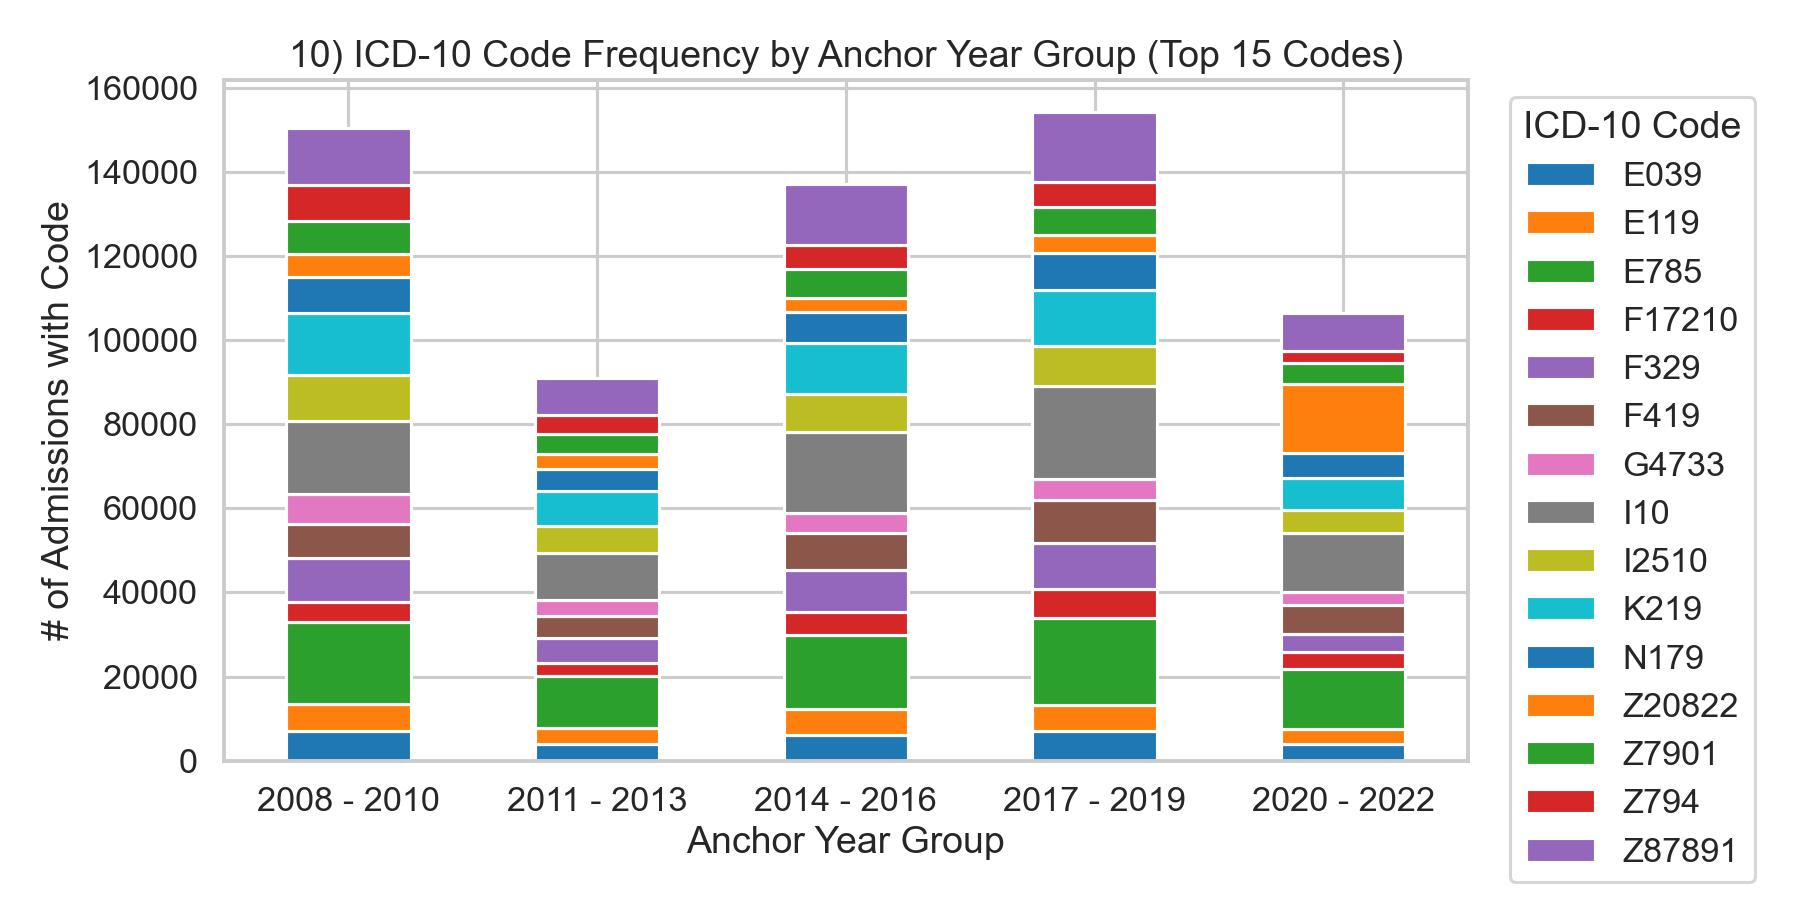
\includegraphics[width=\linewidth]{mimic_plots/plot10.jpg}
    \end{subfigure}\hfill
    \begin{subfigure}{0.54\textwidth}
        \footnotesize
        \textbf{(10) ICD-10 Code Frequency by Anchor Year Group (Top 15 Codes)}\newline
        1) Stacked bars show how often each top-15 ICD-10 code appears per year group.\newline
        2) E785 (hyperlipidemia), I10 (hypertension) remain high across time.\newline
        3) Overall bar heights reflect total admissions with any of these codes in that period.
    \end{subfigure}
    \caption{Left: Stacked bar of top-15 codes across anchor year groups. Right: Description.}
    \label{fig:plot10}
\end{figure}

\section{Key Observations and Implications}
These queries and figures reveal:
\begin{itemize}
    \item \textbf{High Volume of Data:} Over 364k patients and 546k admissions, with \(\sim331k\) discharge summaries available.
    \item \textbf{ICD-10 Emphasis:} \(\sim3.46\)M ICD-10 code assignments vs. \(\sim2.91\)M ICD-9, aligning with modern coding practices.
    \item \textbf{Long-Tailed Codes:} Over 9k ICD-10 codes have fewer than 5 occurrences, underscoring the challenge of rare labels.
    \item \textbf{Multiple Codes per Admission:} An average of 13.6 ICD-10 codes assigned per stay, reflecting a \textit{multi-label} classification problem.
    \item \textbf{Varied Note Lengths:} Discharge summaries range from hundreds to thousands of words, with the top 1\% exceeding 4k words.
\end{itemize}

\section{Final Data Preparation}
\label{sec:final-data-prep}

In order to build a dataset suitable for a scenario akin to AWS Comprehend Medical—where arbitrary clinical text is processed to extract ICD-10-CM codes—we create a single table merging the free-text discharge notes (\texttt{discharge}) with billed ICD diagnoses (\texttt{diagnoses\_icd}), excluding extra demographic fields. This configuration ensures our final text column closely reflects “real world” input, where no additional metadata beyond the raw narrative is guaranteed. 

Concretely, for each hospitalization (\texttt{hadm\_id}), we produce:
\begin{itemize}
    \item A column \texttt{notes}, containing the \textit{unmodified} discharge summary text. 
    \item A column \texttt{icd\_codes}, which is a comma-separated list of all ICD-10-CM codes assigned to that admission.
\end{itemize}

\noindent \textbf{SQL Query:}
\begin{verbatim}
DROP TABLE IF EXISTS mimic.full_notes_with_codes;

CREATE TABLE mimic.full_notes_with_codes AS
SELECT
    d.subject_id,
    d.hadm_id,
    d.text AS notes,
    STRING_AGG(di.icd_code, ',') AS icd_codes
FROM mimic.discharge AS d
JOIN mimic.admissions AS a
  ON d.subject_id = a.subject_id
    AND d.hadm_id = a.hadm_id
JOIN mimic.patients AS p
  ON p.subject_id = d.subject_id
JOIN mimic.diagnoses_icd AS di
  ON di.subject_id = d.subject_id
    AND di.hadm_id = d.hadm_id
WHERE di.icd_version = 10  -- focusing on ICD-10-CM codes only
GROUP BY
    d.subject_id,
    d.hadm_id,
    d.text;
\end{verbatim}


\noindent This final table is readily suitable for a text-to-multilabel model that ingests the discharge narrative in \texttt{notes} and predicts \texttt{icd\_codes}, aligning closely with the use case of free-text medical coding systems.



